%% The first command in your LaTeX source must be the \documentclass command.
%% %% Options:
%% twocolumn : Two column layout.
%% hf: enable header and footer.
\documentclass[
% twocolumn,
% hf,
]{ceurart}


%%
%% Reviewing packages and definitions
\usepackage[dvipsnames,svgnames]{xcolor} % text color
\usepackage[normalem]{ulem} % wavy underlines
\newcommand{\todo}[1]{\noindent\textcolor{red}{{\bf \{TODO}: #1{\bf \}}}}
\newcommand{\TODO}[1]{\todo{#1}}
\newcommand{\citeneeded}{\textcolor{red}{{\bf [?!]}}}
\newenvironment{draft}{\color{gray}}{\color{black}}
\newcommand\jr[1]{{\color{Red}\textbf{JR}: #1}}

%%
%% One can fix some overfulls
\sloppy

%%
%% Minted listings support 
%% Need pygment <http://pygments.org/> <http://pypi.python.org/pypi/Pygments>
\usepackage[outputdir=build]{minted}
%% auto break lines
\setminted{breaklines=true}

%%
%% end of the preamble, start of the body of the document source.
\begin{document}

%%
%% Rights management information.
%% CC-BY is default license.
\copyrightyear{2022}
\copyrightclause{Copyright for this paper by its authors.
  Use permitted under Creative Commons License Attribution 4.0
  International (CC BY 4.0).}

%%
%% This command is for the conference information
\conference{ISWC'23: International Semantic Web Conference,
  November 06--10, 2023, Athens, Greece}


%%
%% The "title" command
\title{Bringing IDE Support to JSON-LD with the Language Server Protocol}

% \tnotemark[1]
% \tnotetext[1]{You can use this document as the template for preparing your
%   publication. We recommend using the latest version of the ceurart style.}

%%
%% The "author" command and its associated commands are used to define
%% the authors and their affiliations.
\author[1]{Author 1}[%
orcid=0000-0000-0000-0000,
]
\author[1]{Author 2}[%
orcid=0000-0000-0000-0000,
]
\author[1]{Author 3}[%
orcid=0000-0000-0000-0000,
]
\address[1]{Some place on the world}


%%
%% The abstract is a short summary of the work to be presented in the
%% article.
\begin{abstract}
  JSON-LD is a popular data format used to describe and share semantic data on the web.
  However, creating and editing JSON-LD documents can be a challenging task, especially when dealing with complex contexts that include many properties.
  The existing JSON editing functionality may not suffice for developers, and a JSON-LD editor could greatly enhance their experience.
  In this paper, we introduce a JSON-LD Language Server based on the Language Server Protocol (LSP) that empowers text editors compatible with the LSP (e.g., Visual Studio Code and NeoVim) with IDE functionality, including autocompletion suggestions based on the defined context, semantic highlighting and renaming identifiers inside the document.
  We believe that a JSON-LD LSP will enhance developer ergonomics and promote its adoption.
  Moreover, we see high potential for additional features that can be added such as hovering, go-to-definition and code actions like flattening or structuring of JSON-LD documents.
\end{abstract}

%%
%% Keywords. The author(s) should pick words that accurately describe
%% the work being presented. Separate the keywords with commas.
\begin{keywords}
  Linked Data \sep 
  JSON-LD \sep
  Developer UX \sep
  Tool \sep
  Language Server
\end{keywords}

%%
%% This command processes the author and affiliation and title
%% information and builds the first part of the formatted document.
\maketitle

\section{Introduction}

JSON-LD is a data serialization format that is used to describe semi-structured data on the web\cite{JSON-LD-W3C}.
It adds semantic information to JSON, among others with the \textit{@context} property, pointing to a JSON-LD context.
This context specifies how to map properties to predicates, called aliases.

With its increasing popularity, contexts in JSON-LD also increase in complexity.
For example, the Flemish (Belgium) OSLO initiative is working to achieve interoperability by building semantic standards for different stakeholders such as government, industry and academia\footnote{\href{https://www.vlaanderen.be/digitaal-vlaanderen/onze-oplossingen/oslo}{OSLO} - Open Standaarden voor Linkende Organisaties}.
They focus on standardizing JSON-LD context files for their vocabularies and application profiles. 
An example is \href{https://data.vlaanderen.be/doc/applicatieprofiel/vlaamse-codex/}{the Flemish codex application profile}, the context defined for this profile enables JSON objects with Dutch properties to be interpreted as linked data.

Another example where JSON-LD contexts are extensively used is the semantic dependency injection framework ComponentsJs\cite{CJS}. 
ComponentsJs allows Javascript packages to define JSON-LD contexts that describe the package, these contexts are then used to configure and instantiate an application.

Creating new JSON-LD documents is a difficult task, before the developer knows the defined aliases, he has to scrupulously explore the context and remember the defined names. 
Accidental typos can result in broken linked data and to the best of our knowledge, there are no tools in existence that could assist in preventing this issue.
We show that using a language server for JSON-LD helps alleviate this problem and can also bring better developer ergonomics for experienced and new semantic web developers.

Similar efforts have been made before, but never for JSON-LD. 
For example, the Yasgui editor\footnote{\href{https://triply.cc/docs/yasgui/}{Yasgui} - SPARQL editor}, a popular SPARQL human query interface, provides autocompletion based on the LOV API\cite{LOV}. 
Plugins can also add autocompletion based on domain knowledge. 
These capabilities are built into the deployed editor and can only be used with Yasgui.
Stardog created open-source LSPs for turtle, TRIG, SPARQL, and more, however, they focus only on correct syntax and keyword auto-completion\cite{stardog}. 

In this paper, we introduce a JSON-LD language server implementation following the Language Server Protocol (LSP), a JSON RPC protocol designed by Microsoft\footnote{\href{https://microsoft.github.io/language-server-protocol/}{LSP}}.
LSP is designed to simplify the process of integrating language-specific logic into an editor, removing the need to implement language-specific logic into each editor, and reducing the \(O(n*m)\) complexity to a much more manageable \(O(n+m)\) complexity\cite{LSP-Multi}.

A full LSP implementation supplies the editor with IDE features, including autocompletion, diagnostics, formatting, identifier renaming, hovering, go-to-definition and generic code actions like \textit{extract highlighted code to function}. 
Not all features have to be implemented, the Language Server and the editor communicate their capabilities and only use what is supported by both parties.

All source code of the demo and installation instructions are available on GitHub (MIT).


\section{Features of the JSON-LD language server}

% The Language Server Protocol (LSP) is a JSON RPC protocol developed by Microsoft to simplify the process of integrating language-specific logic into an editor\footnote{\href{https://microsoft.github.io/language-server-protocol/}{LSP} - Language Server Protocol}. 
% Before LSP, editors had to implement each programming language they wanted to support individually, resulting in an \(O(n*m)\) complexity, where n is the number of editors and m is the number of programming languages.
% With LSP, editor and language-specific logic only need to be implemented once, resulting in a much simpler \(O(n+m)\) complexity\cite{LSP-Multi}.
% LSP only concerns itself with the source files of the program and doesn't involve building, running, or debugging.
% This is in contrast to the Build Server Protocol \footnote{\href{https://github.com/build-server-protocol/build-server-protocol}{BSP} - Builder Server Protocol}.

This section covers what features are implemented, how and what benefit they provide the developer.

\begin{itemize}
  \item \textbf{Autocompletion} enables the developer to type less and thus make fewer mistakes.
    The created suggestions are derived from the defined context\footnote{Only simple and explicit aliases are extracted from the context, context overloading or scoped contexts are not supported.} and defined entity ids inside the document.
    This way developers don't have to remember aliases by heart and can more easily explore the context.
    An example can be seen in Figure \ref{fig:complete}.
    It should be possible to write \textit{foaf:} and get autocompletion suggestions for all defined predicates in the \textit{foaf} namespace, but this is not yet supported.
  \item \textbf{Diagnostics} represent errors and warnings in the file.
    Our language server only supports syntax errors but emitting a warning when an undefined property is encountered, can be an easy extension.
  \item \textbf{Semantic Highlighting} differs from syntax highlighting.
    The syntax of JSON-LD is very easy, but semantic highlighting highlights keywords, identifiers and tokens differently.
    Other semantic highlighting functionality includes highlighting defined/undefined properties and highlighting entity ids and types, these are however not implemented.
  \item \textbf{Renaming}, in our LSP, allows the developer to rename defined identifiers and their references.
    An example of renaming an entity can be seen in Figure \ref{fig:rename}, first the editor will ask for a new name, then all occurrences are renamed.
    % These code actions can also be extended to enable flattening, compacting or expanding of the entire document, but are not supported in the current implementation.
  % \item \textbf{Hover} can show additional information about properties. By using the power of linked data, the IDE can dereference the property and look for some description of the used property.
\end{itemize}

\begin{figure}
\centering
\makebox[\textwidth][c]{
    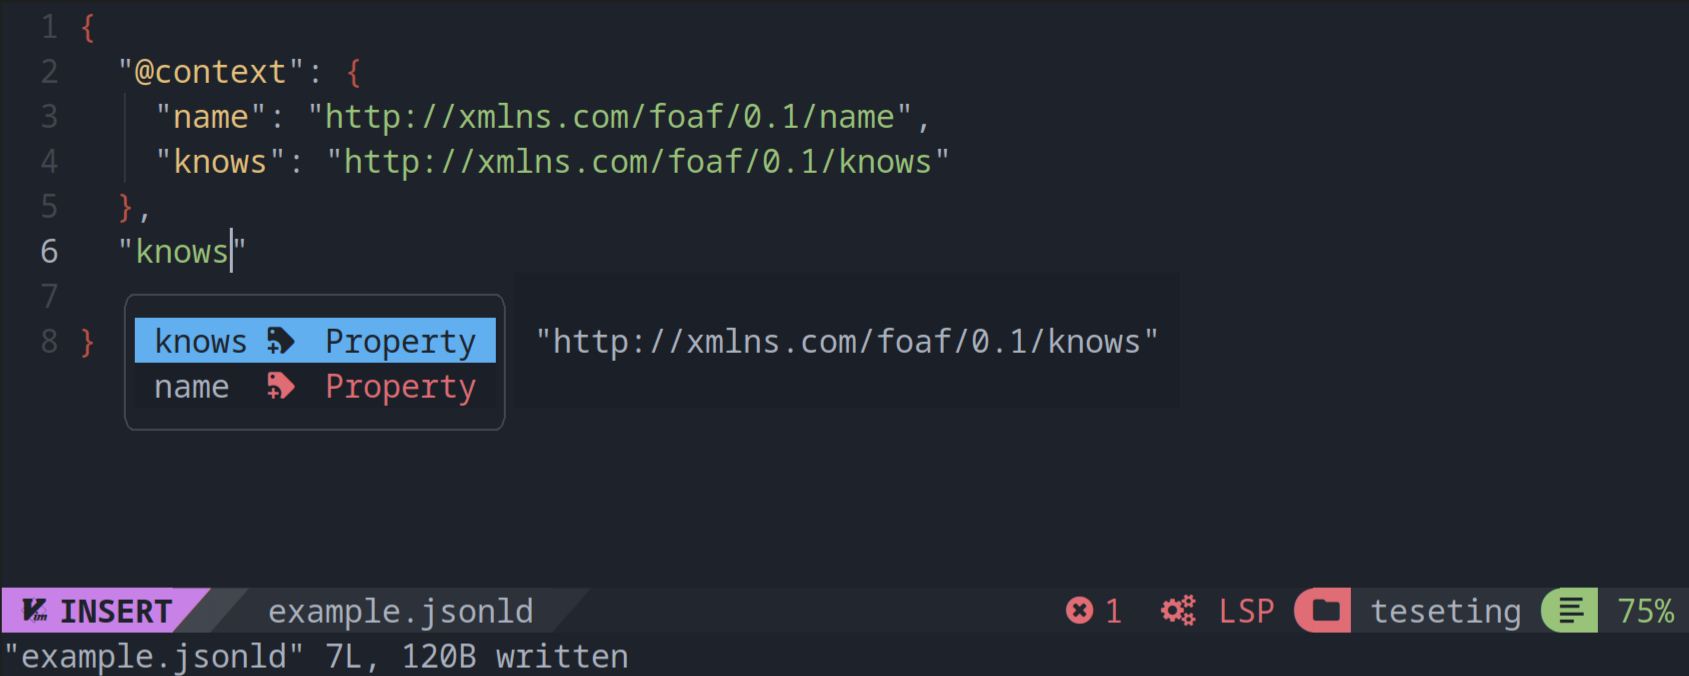
\includegraphics[width=.5\linewidth]{./fig/completion.png}
    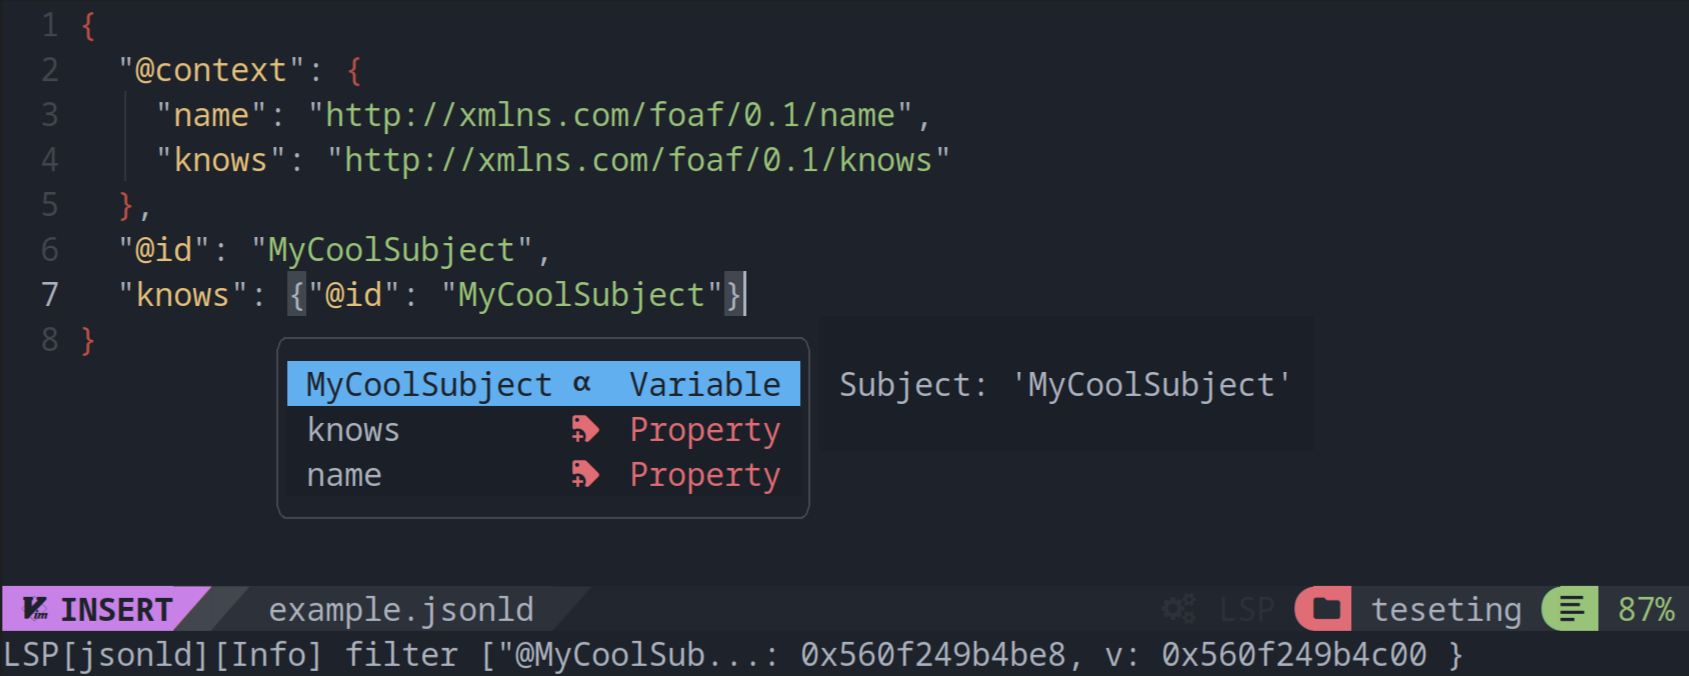
\includegraphics[width=.5\linewidth]{./fig/completion-id.png}
}
\caption{Screenshots showing completion functionality in NeoVim: the left side shows completion suggestions, and the right side also shows defined identifiers.}
\label{fig:complete}
\end{figure}


\begin{figure}
\centering
\makebox[\textwidth][c]{
    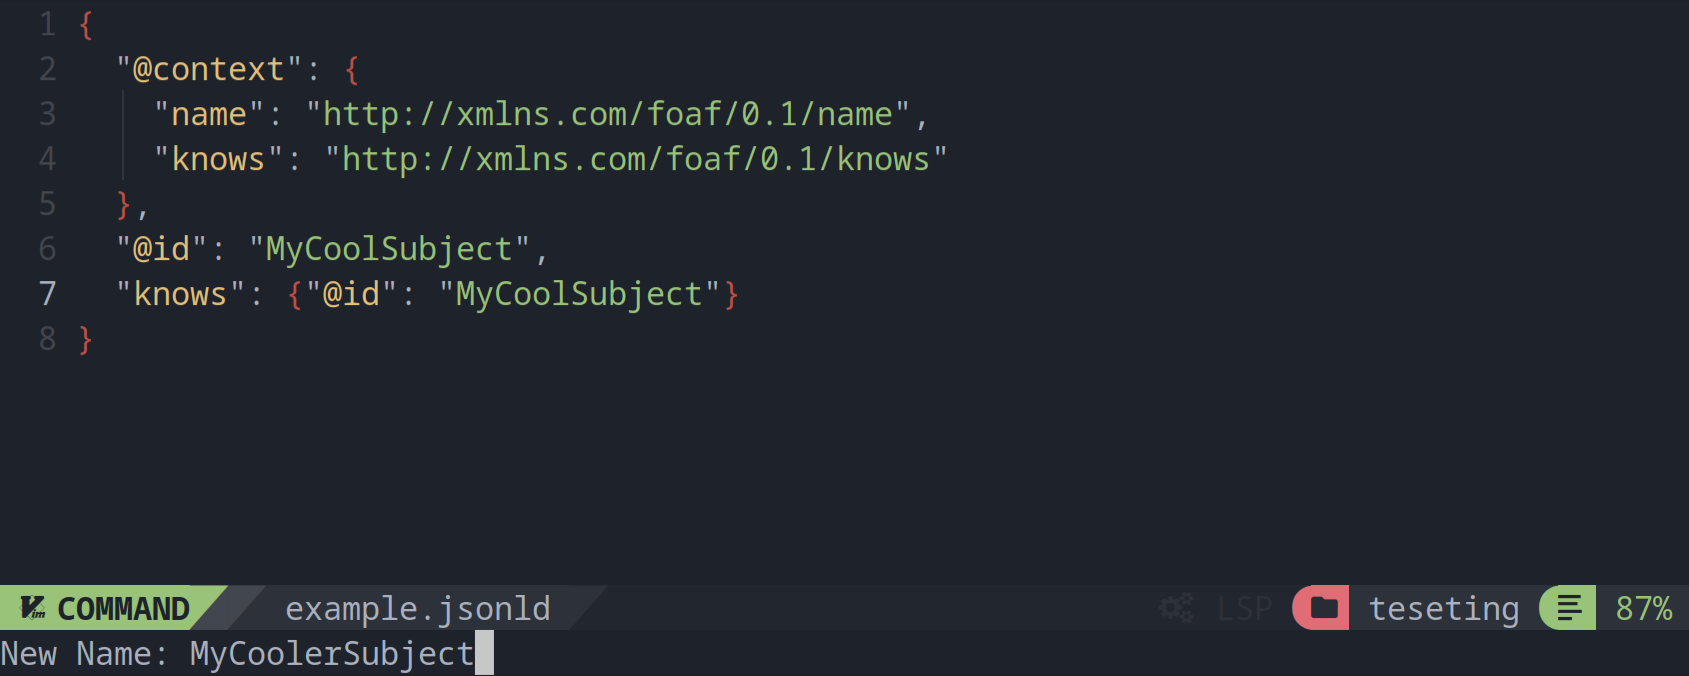
\includegraphics[width=.5\linewidth]{./fig/rename-1-small.png}
    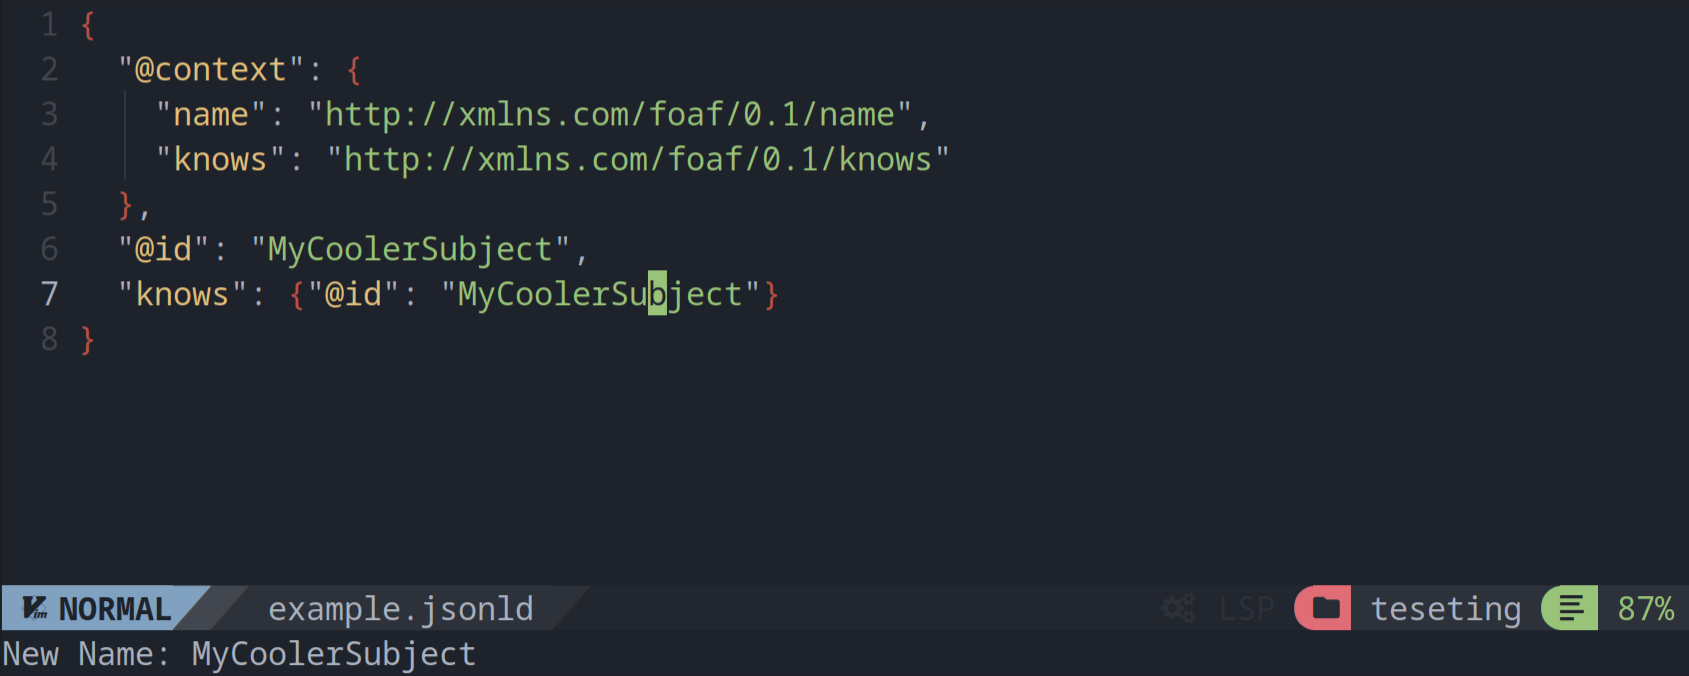
\includegraphics[width=.5\linewidth]{./fig/rename-2-small.png}
}
\caption{Screenshots showing renaming functionality in NeoVim: left NeoVim asks for the new name, right the subject is renamed.}
\label{fig:rename}
\end{figure}


\section{Demo}

Our demo presents an implementation of a JSON-LD Language Server according to the Langauge Server Protocol (LSP), developed using the Rust programming language based on a basic LSP implementation\footnote{\href{https://crates.io/crates/tower-lsp}{Tower LSP} - Crate by Eyal Kalderon}.
The full source code and installation instructions can be found on GitHub (MIT).
A demo version of the LSP is available on the \href{https://jsonld.tiiny.site/}{web}\footnote{Slimmed down and anonymized version for reviewing purposes}.
The full LSP is available as a VS Code extension and as a NeoVim LSP.

The Language server is compiled to WASM to be integrated inside the VSCode extension.
This enables the extension to be a Web Extension\footnote{https://code.visualstudio.com/api/extension-guides/web-extensions} is available in online Visual Studio Code instances like \textit{github.dev}.

Extracting predicate mappings from the context is handled by the JSON-LD crate\footnote{\href{https://crates.io/crates/json-ld}{JSON-LD} - Crate by Timothée Haudebourg}.
Some parts of the JSON-LD crate can't compile to WASM, because of internal Rust requirements\footnote{Fetching a resource in WASM is not \textit{Send} or \textit{Sync}, which is required in \textit{async} environments} and required some rewriting of the crate. 

Parsing the JSON structure is done with the Chumsky crate\footnote{\href{https://github.com/zesterer/chumsky}{Chumsky} - Crate by Joshua Barretto}.
This was no easy task because the moment the Language Server should suggest completion options, the document is no valid JSON anymore. 
This required a special internal JSON structure allowing parts of a dictionary to be invalid.


\section{Conclusion}

This JSON-LD LSP is an example of what impact developer tools can have on productivity and therefore also on adoption.
The same ideas can be applied to other semantic data formats to help write but also, with hover functionality, to help understand the data more easily. 

This demonstration merely scratches the surface of the vast capabilities of a JSON-LD LSP.
By leveraging fully-interpreted contexts, the LSP can provide more contextually-relevant suggestions, taking into account context overloading and scoped contexts. 
Additionally, the LSP's functionality can be expanded to include the interpretation of referenced vocabularies, allowing completion for compacted predicates, like \textit{foaf:knows}.
Despite its current limitations, the LSP already enhances the developer experience by facilitating the creation and editing of JSON-LD documents.

On the development side, this demo contributes to the open-source community. 
There are not many examples of Language Servers written in Rust and compiled to WASM to be included in a Visual Studio Code extension.
Hopefully, this implementation starts a cascade of developer tools for the semantic web community.


%%
%% Define the bibliography file to be used
\bibliography{bibliography}


\end{document}

%%
%% End of file

